% !TeX spellcheck = pl_PL-Polish
\documentclass[12pt,a4paper]{article}

\usepackage[T1]{fontenc}
\usepackage[polish]{babel}
\usepackage[utf8]{inputenc}
\usepackage{lmodern}
\selectlanguage{polish}
\usepackage{graphicx}
\usepackage{xcolor}

\def\projectName{Moduł Który Stworzyliśmy}
\def\authorA{Beniamin Stecuła}
\def\authorB{Benjamin Stecula}
\def\authorC{Benĉjo Stecuŭa}
\newcommand\todo[1]{\textcolor{red}{#1}}

\begin{document}
\pagenumbering{gobble}
\clearpage
	\begin{figure}[h]
		\centering
		%
\includegraphics[width=0.5\linewidth]{media/polsl_logo_pion_en_rgb.png}
		
\includegraphics[width=0.5\linewidth]{media/ps-logo.png}
	\end{figure}

\hspace{3cm}
	\begin{center}Dokumentacja projektowa\end{center}
	\hspace{3cm}
	\begin{center}\large\textbf{Zarządzanie Systemami Informatycznymi}\end{center}
	\begin{center}\large\textit{\projectName}\end{center}

\hspace{7cm}
	\begin{flushright}Kierunek: Informatyka
		\end{flushright}
		\begin{flushright}Członkowie zespołu:
		\par
		\textit{\authorA}
		\par
		\textit{\authorB}
		\par
		\textit{\authorC}
	\end{flushright}
\vfill
	\begin{center}Gliwice, 2025/2026\end{center}

\newpage
\pagenumbering{arabic}
\tableofcontents





\newpage
\section{Wprowadzenie}
\subsection{Role w projekcie}
	\ldots 

\subsection{Cel projektu}
	\begin{figure}[h]
		\centering
		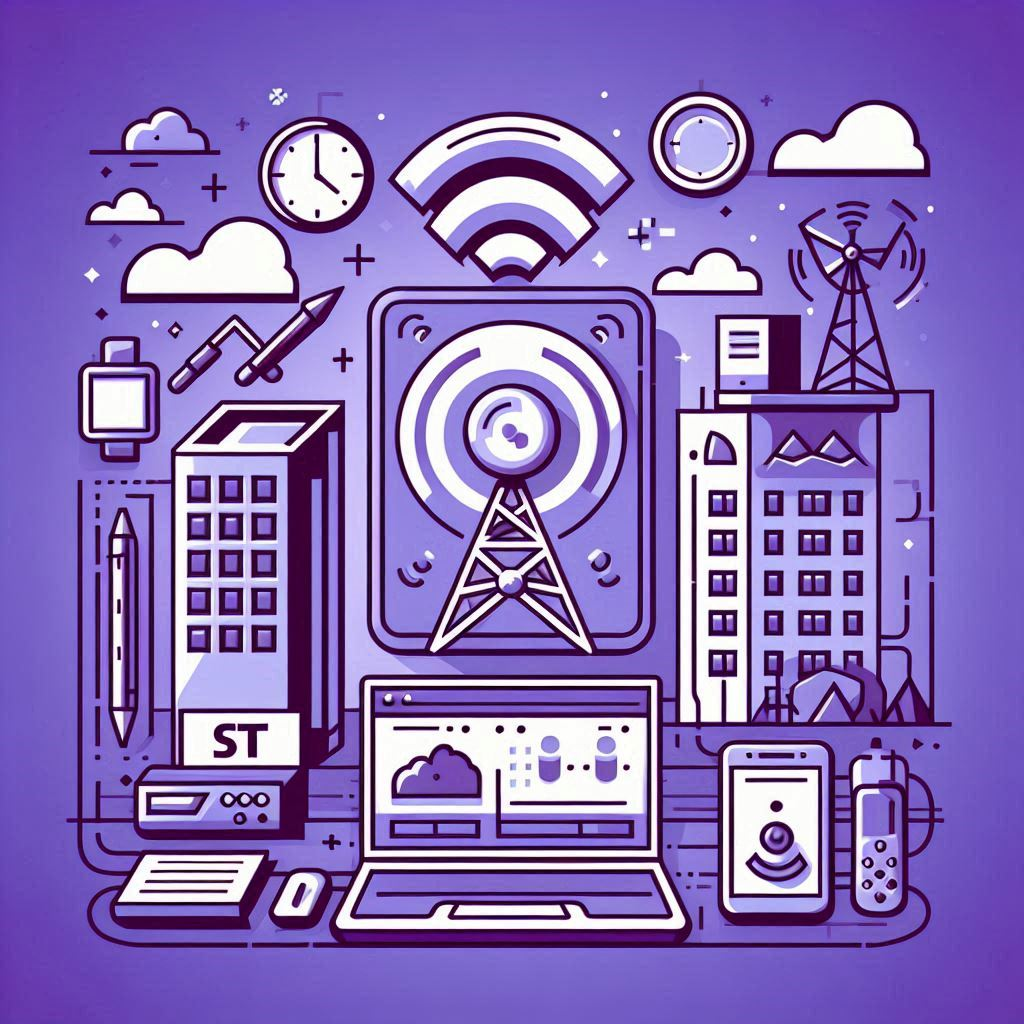
\includegraphics[width=0.5\linewidth]{media/logo_ZSI.jpeg}
		\caption[LogoZSI]{Logo Projektu}
		\label{fig:logo_ZSI}
	\end{figure}
	Celem projektu jest \todo{stworzenie projektu}. \\
	\ldots 





\newpage
\section{Założenia projektowe}
\subsection{Założenia techniczne i nietechniczne}
	\ldots 

\subsection{Stos technologiczny}
	Narzędzia i systemy informatyczne związne z projektem

\subsection{Oczekiwane rezultaty projektu}
	\ldots 





\newpage
\section{Realizacja projektu}
	Opis wszystkich etapów realizacji projektu. \\
	Ilustrujemy licznymi \todo{zdjęciami i grafikami}. \\





\newpage
\section{Wnioski}
	\begin{itemize}
		\item \textit{Spostrzeżenia}
		\item \textit{Osiągnięcia}
		\item \textit{Potencjał rozwoju}
	\end{itemize}





\newpage
\section{Bibliografia}
\begin{enumerate}
	\item Internet
\end{enumerate}

\end{document}